\begin{frame}[fragile]{Funktion random\_exp(n, p)}
  \begin{columns}
  \column{.49\textwidth}
    \begin{itemize}
  	\item Erzeugt exponential verteilte Zufallszahl
  	\item Gemäß Inversionsmethode:
  	\item $ZZ = -\frac{1}{\lambda} ln(u)$ mit u=R(0,1)
  \end{itemize}
  \begin{lstlisting}[language=python]
def random_exp(lambd):
    rand = random.random()
    return -(1/lambd) * log(rand)
\end{lstlisting}
\logopythonbottom
  \column{.49\textwidth}
    	\begin{figure}[h!]
    	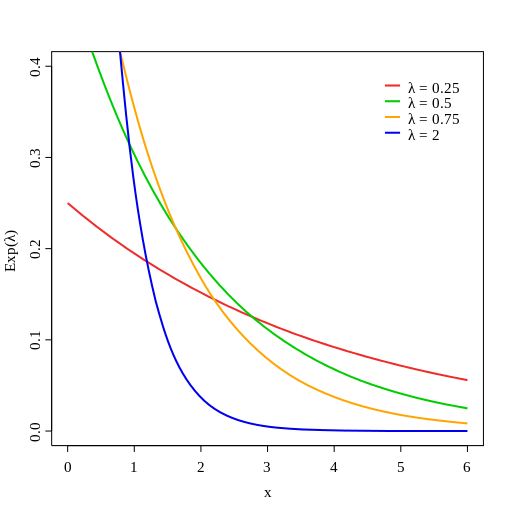
\includegraphics[scale=0.3]{lib_random_exp_wahrscheinlichkeitsverteilung.png}
  			\caption{Wahrscheinlichkeitsverteilung der Exponentialverteilung \tiny{(Wikipedia)}}
		\end{figure}
  \end{columns}
\end{frame}	